\listfiles
\documentclass[english,blauw]{cbsdiscussionpaper}

%%% PACKAGES

% These packages are all incorporated in the memoir class to one degree or another...
\usepackage[english]{babel}
\usepackage{graphicx} % support the %\includegraphics command and options
\usepackage{booktabs} % for much better looking tables
\usepackage{array} % for better arrays (eg matrices) in maths
\usepackage{verbatim} % adds environment for commenting out blocks of text & for better verbatim
\usepackage{subfig} % make it possible to include more than one captioned figure/table in a single float
\usepackage[authoryear]{natbib}
\usepackage{float}
\bibliographystyle{chicago}

%%% The "real" document content comes below...

\title{Filtering in the Fourier domain: a new set of filters for seasonally adjusted time series and its evaluation}
\author{Eugenio Perrucci \& Frank Pijpers}
\Number{2016}{05}
\Sector{Sector Procesontwikkeling en Methodologie (BPM)}
\Projectnummer{12345678}
\Keywords{time series analysis, X12-ARIMA, TRAMO-SEATS, Fourier transform}
%\AdresDenHaag


%%% HEADERS & FOOTERS
%\usepackage{fancyhdr}% This should be set AFTER setting up the page geometry
%\pagestyle{fancy} % options: empty , plain , fancy
%\renewcommand{\headrulewidth}{0pt} % customise the layout...
%\lhead{}\chead{}\rhead{}
%\lfoot{}\cfoot{\thepage}\rfoot{}

%%% SECTION TITLE APPEARANCE
%\usepackage{sectsty}
%\allsectionsfont{\sffamily\mdseries\upshape} % (See the fntguide.pdf for font help)
% (This matches ConTeXt defaults)

%%% ToC (table of contents) APPEARANCE
%\usepackage[nottoc,notlof,notlot]{tocbibind} % Put the bibliography in the ToC
%\usepackage[titles,subfigure]{tocloft} % Alter the style of the Table of Contents
%\renewcommand{\cftsecfont}{\rmfamily\mdseries\upshape}
%\renewcommand{\cftsecpagefont}{\rmfamily\mdseries\upshape} % No bold!

%%% END Article customizations

\begin{document}
\maketitle

\tableofcontents
\clearpage

\begin{abstract}
The identification and removal of the seasonal component is one of the main issues in time series analysis, and it is a key operation performed by national statistical agencies such as Statistics Netherlands. Several procedures exist for this goal, available in a wide range of software. The most often applied techniques are based on the use of filters.  A linear filter is proposed in this paper, which can be incorporated in existing frameworks and packages for the treatment of time series, and which identifies seasonal influences in one step, with no iteration required. The aim of the study is to evaluate the efficacy of this proposed filter. In particular, the filtered series is used as the input of a seasonal adjustment procedure, performed by JDemetra+. This latter is a software for time series seasonal adjustment recommended by the European Statistical System (ESS) and European System of Central Bank (ESCB). It incorporates two methods: X-13-ARIMA, an enhanced X-11 seasonal adjustment procedure (see \citep{can1980}), developed by the U.S. Census Bureau, and TRAMO/SEATS (see \citep{margo1997}, and \citep{marsa2000}), proposed by the Bank of Spain. The performance of the proposed filter is analyzed on a real time series; most of the observed diagnostics focus on spectral analysis.
\end{abstract}
\section{Introduction}
A key concept in time series analysis is the decomposition of a given time series into a trend component, a seasonal component and noise. Seasonality consists in movements repeated throughout the year, with similar intensity in different years. It means that they are expected to be predictable. Seasonal movements are often large enough such that they can mask other characteristics of the data that are of interest to analysts of current trends. Removal of the seasonal component allows to produce series whose movement are easier to evaluate over time. Indeed, seasonal movements can arise with different timing and amplitude for different time series, complicating their comparison in trend-cycle terms. In a series free of seasonal movements, it is also easier to achieve better forecasts.
\begin{figure}[h]
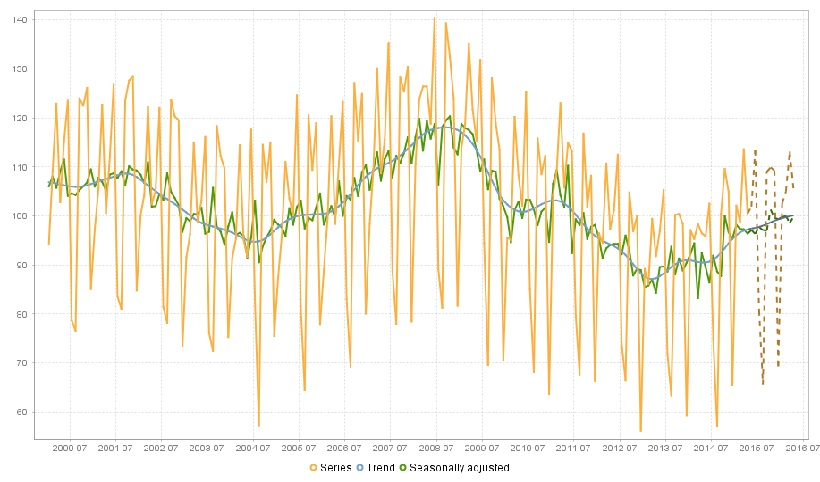
\includegraphics[width=\linewidth]{../images/capitolo1/intro.jpg}
\caption{A decomposition of the Netherlands volume index of production time series in trend and seasonally adjusted series performed by JDemetra+.}
\label{fig:intro}
\end{figure}
Figure \ref{fig:intro} shows a decomposition of a time series obtained through a JDemetra+ seasonal adjustment procedure. A common method for obtaining the trend is to use linear filters on given seasonally adjusted series, and in the simplest case moving averages are considered. It means that the filtered value at time $t$ is an average of the values in a neighbourhood of pre-defined length of that target point. The most often applied filters used to estimate the trend-cycle are the Henderson filters (Henderson, 1916). It is the most widely applied filter to estimate the trend-cycle component in nonparametric seasonal adjustment software, such as the U.S. Bureau of the Census X-12-ARIMA and its variant, X-13-ARIMA. For a good overview of recent developments about capabilities of this software see \citep{fin2005} and references therein. Those procedures are also available in other software, like Gretl, R, EViews, and, particularly, in JDemetra+.\\
This latter is  a statistical software package for seasonal adjustment supported by Eurostat. It includes two methods: X-13-ARIMA and TRAMO/SEATS. Both of the procedures imply a similar pre-treatment of the time series, aimed to fit an ARIMA model (called RegARIMA) to historical data; after evaluating the deterministic effects, such as outliers, Easter effects, trading days, leap years etc. etc.), and including them in the RegARIMA regression model. The two procedures strongly differ in how the time series decomposition is performed. As mentioned before, X-13-ARIMA works with nonparametric linear filters, while TRAMO/SEATS estimates the various components with signal extraction techniques based on ARIMA models, specified for each component of the series (a detailed discussion is offered by \citep{mar2008}). The estimation of the model parameters is done using the so called Weiner-Kolmogorov filters.\\
Another relevant topic related to time series analysis is the revisions problem. Many variables, published at sub-annual frequency (monthly or quarterly), produce new data continuously. An effect of this is that the current or most recent observations are subject to revisions as new observations become available. This is because asymmetric filters are usually used to smooth the last observations. These filters are time-dependent, i.e. there is a different one for each of the last time points. Therefore, as new observations are available, the estimate of the previous observation is modified, because it is re-calculated with a different filter. Then, the seasonally adjusted series need to be updated. Those updates are called revisions. A considerable disadvantage of the available procedures is that revisions produce usually entirely new seasonal adjusted time series. While in practice the updates on older sections of the adjusted time series may be minimal, it is unsatisfactory not to be able to regard any part of the time series as definitive or final. The question is how to reduce the frequency of revisions without losing accuracy in estimation. For a further discussion of the asymmetric filters problem, see \citep{dageal2015}.
The paper is structured as follows. Section 2 decribes the proposed filter and discusses its properties in the frequency domain. Section 3 reports a seasonal adjustment procedure carried out on a real time series, characterized by a strong seasonal influence. The analysis is performed using JDemetra+, and it focuses on the spectral analysis of the input and  of the output of the seasonal adjustement. After filtering the time series using the proposed filter, in Section 4 the filtered series is used as the input of JDemetra+,  to assess whether the removal of the seasonal component obtained by the filter is satisfactory or not.\\
\section{Filters in the time domain and the Fourier domain}
For a thorough discussion of the effects that a general filter has on a time series, a valuable diagnostic is the frequency response of that filter. The latter consists in the Fourier transform of the filters factors. The Fourier transform is often also referred to as the Fourier spectrum.\\ 
\subsection{The Fourier transform}
The Fourier transform Y $(\omega)$ of a function of time \textit{y}(\textit{t}) is:
\begin{equation}
Y (\omega)\equiv \mathcal{F} (\textit{y})= \int \ e^{i \omega t} y(\textit{t}) dt
\end{equation}
with
\begin{equation*}
e^{i \omega t} \equiv \cos(\omega t) + i \sin(\omega t)
\end{equation*}
Here $\omega$ is the frequency of a signal, related to the period \textit{P} by:
\begin{equation}
\omega = \frac {2\pi}{P}
\end{equation}
For the Fourier transform there is also an inverse operation.
\begin{equation}
y(\textit{t}) = \mathcal{F}^{-1} (Y) = \frac {1}{2 \pi} \ \int d\omega \ e^{-i \omega t} Y(\omega)
\end{equation}
One property of the Fourier transform, that will be useful for the further discussion, is that it is a linear operation, and therefore so are the inverse operations. Linearity implies that the Fourier transform of the sum of functions \textit{y}(\textit{t}) and \textit{z}(\textit{t}) is the sum of their Fourier transforms \citep{bracewell1965}:
\begin{equation}
\mathcal{F}(\textit{a} y + \textit{b} z) = \textit{a} \ \mathcal{F}(y)+ \textit{b} \ \mathcal{F}(z)
\end{equation}
where \textit{a} and \textit{b} can be any constant.\\
If the function \textit{y}(\textit{t}) is only known at discretely sampled times \textit{t$_i$}, which are regularly spaced, a discrete version of the Fourier transform can be defined as well, where the integral is replaced by summation with appropriate weights for each of the samples \textit{y$_t$}, as follows:
\begin{equation}
\mathcal{F}(y) = \sum_t  \ e^{i \omega t} y(\textit{t})
\end{equation}
This paper will refer to \textit{y$_{ti}$} with \textit{y$_t$}. Since there are particularly efficient algorithms (the Fast Fourier transforms or FFTs) for computing discrete Fourier transforms if the number of samples is exactly a power of 2, normally time series are truncated to an appropriate length or padded out symmetrically with appropriate average values in order to get the number of samples which satisfies this criterion. A useful reference for FFT implementations and their properties is \citep{presea1992}.\\Of particular importance when carrying out discrete Fourier transforms is a limitation that is imposed by the sampling cadence, which is the time interval between consecutive observations. Indeed, with a finite cadence of sampling, with time interval $\Delta_t$, it is impossible to detect any periodic signal with a frequency that is higher, in absolute value, than the Nyquist frequency. The latter is:
\begin{equation}
\omega_{N_{yq}} = \frac {\pi}{\Delta_t}
\end{equation}\\
The Nyquist frequency is related to the total length of the considered period T, in the following manner:
\begin{equation*}
\begin{split}
T=N\Delta_{t,}\quad \quad \Delta_{t}=\frac{T}{N},\quad \text{and so:} \quad \omega_{Nyq}=\frac{\pi N}{T}
\end{split}
\end{equation*}
where N is the number of observations.\\
A discretely sampled finite time series can be represented without loss of information by its discretely sampled Fourier transform. Since the Fourier transform or spectrum is complex valued, the number of sampling points required is only half the number of points in the time series. If a standard FFT is applied on a time series, these sampling points are uniformly spaced over the frequency interval\ $[0,\omega_{Nyq}]$.\\The reason for discussing Fourier transforms in the context of filtering a time series is that filtering in the time domain corresponds to a particularly simple operation in the frequency domain. In general, filtering in the time domain of a regularly sampled time series can be written in the form of a weighted average:
\begin{equation}
\tilde {y_t} = \sum\limits_{k=-m}^{n} \textit{w$_k$}\textit{y$_{t+k}$}
\end{equation}
where the weights \textit{w$_k$} are the filter factors. This is a general form, allowing for asymmetric filtering. For instance, in causal filters, $n=0$, so that only information from the previous and present observations of a time point is used and none from the successive ones (this is necessary when estimating time series components in the last time point available). While \textit{m} and/or \textit{n} could in principle be infinite, this has no practical purpose in the current context. Also, in the context of seasonal filtering it is more usual to employ symmetric filters so that not only $m=n$ but also $w_{-k} = w_k$. Often an additional property imposed is that $\sum w_k = 1$, but in the applications at hand this is not always used. \\ The equation (7) above is known as a convolution in the time domain of the function \textit{y} and the function \textit{w}, in which the latter is simply the set of averaging weights interpreted as (samples of) a function of time. It can be demonstrated that the Fourier transform of the convolution of two series in the time domain is identical to the product of the Fourier transforms of the two series \citep{bracewell1965}. Therefore the Fourier transform of the filtered time series $\textit{\~ y}$ can be calculated as the product of the Fourier transform of the original time series and the Fourier transform of the filter function \textit{w}.
\begin{equation}
\mathcal{F}(\tilde {y}) = \mathcal{F}(y * w) = \mathcal{F}(y)\mathcal{F}(w)
\end{equation}
in which the * indicates the convolution of functions. Multiplication is a much more straightforward operation than calculating the above running averages of (7), and in the frequency domain it is also more straightforward to see the effect of a filter on a signal with a particular frequency or period. In the paper of \citep{dageal1996} the frequency domain properties of many of the filter choices of the X11-ARIMA package are discussed in detail, which remain valid also for the most recent X12 implementations.\\ This suggests an alternative approach to create a set of weights, namely by starting with some desirable properties of the filter in the Fourier domain, and then inverse transforming to obtain the appropriate weights \textit{w$_k$}.\\
\subsection{ Designing an improved filter}
Determining the effect that a particular set of weights has in the frequency domain is useful to design of a set of weights that is in some sense ``optimal''. In practical operations, such as those performed by eg. Statistics Netherlands, the intention is to regularly publish or update seasonal adjusted time series and perhaps also the time series of seasonal factor. In this case it may be useful to apply a moving average in the time domain, rather than Fourier transforming the entire time series, carrying out the multiplication in the frequency domain and subsequently inverse transforming again. Useful discussions of the spectral analysis of time domain filters can be found for instance in \citep{gre1970},\citep{shueal2011} and \citep{fineal2006}.\\In designing the weights it is advisable  to have the total extent of non-zero values \textit{w} as limited as feasible, ie. to make \textit{m} and \textit{n} in equation (7) as small as possible.
\begin{equation}
w_k \equiv 0 \quad \forall |k| > max(m,n).
\end{equation}
The reason for this is that when updating the published seasonal adjusted time series, only the most recent samples need to be flagged as provisional, whereas further back beyond the $m^{th}$ sampled point in the past the seasonal adjusted series can be considered final, because by design it can no longer change in any regular update.\\A separate desirable feature is for the Fourier transform of \textit{w} to have zero imaginary part, $\mathfrak{F}(W) = 0$, so that the phase of periodic signals is unaffected by the filtering operations. For the Fourier transform of \textit{w} to be entirely real, the weights \textit{w} need to be symmetric around 0. For this reason the design will focus on symmetric weights for which:
\begin{equation}
w_{-k} = w_k
\end{equation}
Another requirement is that the long-term average of the seasonal component has to be equal to 0. Translated to the frequency domain, it means that the value of the Fourier transform of the seasonal component at $\omega=0$ must be equal to 0. The Fourier transform of the original time series can have any value, so by making use of equation (8) it can be seen that this requirement can be met if the Fourier transform $W(\omega)$ of the weights \textit{w} for isolating the seasonal component is equal to 0 at $\omega=0$.  Translating the requirement $W(0)=0$ back to the time domain yields the simple constraint that:
\begin{equation}
\sum \limits_{k=-n}^n w_k \equiv 0
\end{equation}
If the weights \textit{w} are designed to determine the seasonal component, the \textit{trend+cycle+noise} series can be obtained by subtracting the seasonal component from the original time series. This is the case of the set of filter weights proposed  here. The linearity property (4) ensures that such additions and subtractions in the time domain are treated identically in the frequency domain. If one has a filter W($\omega$) in the frequency domain which is designed to extract seasonal movements from a time series, then the filter 1 - W produces a time series with just the \textit{trend+cycle+noise}. This implies that there is an additional desirable property or (soft) constraint for the values $W_k$ in the frequency domain which is that:
\begin{equation}
-\epsilon < W_k < 1+\delta
\end{equation}
in which $\epsilon$ and $\delta$ are as small as feasible given the other constraints. While ideally $\epsilon=0$ and $\delta=0$, in practice with a finite set of filter weights \textit{w} satisfying (9), this may not be achievable. This implies that if the dynamic range of the original time series is very high (ie. the height $h_f$ of a peak in the Fourier transform of the time series is very large) there may still be undesirable remaining seasonal signal in the filtered time series, because $\delta h_f$ and/or $\epsilon h_f$ are not sufficiently small.\\The standard filtering procedures involved in TRAMO/SEATS and X-13-ARIMA imply an assumption or idealisation that the seasonal movements in a time series are perfectly periodic and repeat identically from one year to the next. If this were indeed the case, then it would be perfectly adequate to design weights that eliminate signal at very specific frequencies that are integer values in the units of cycle/years. The weights of this standard approach, when Fourier transformed, produce the graph shown in Figure \ref{fig:filters} (dashed line). It clearly shows notches precisely at integer multiples of 1 cycle/year, broadened because of the finite resolution of the sampling in the frequency domain.\\
The problem with standard filtering is that signal that is not precisely at these frequencies but in-between, is not included in the seasonal effect. For a real time series this genuinely causes issues because in practice also the ``envelope'' of the seasonal effect is subject to long term changes. The seasonal pattern may qualitatively be very similar from year to year but most often it will not be completely identical from one year to the next: eg. the amplitude may be well modulated by effects similar to those that determine long-term trends or economic cycles. Such long term effects on seasonal patterns have a signature in the frequency domain: strong peaks at integer multiples of one cycle/year will be substantially broadened, and therefore produce signals at frequencies where the filter corresponding to the naive design of the standard procedures will not include them in the seasonal component and, therefore, also not extract them from the \textit{trend+cycle+noise} series.\\For this reason it is more suitable for real time series to design a filter that ``removes'' all signal in a band between frequencies of around one cycle/year ie. between $\sim$ 1/12 cycle/month and $\sim$ 5/12 cycles/month. In the context of smoothing a monthly input, the frequency domain $\Omega=(0<\frac {\omega}{2\pi}<0.5)$ can be portioned in two main intervals: (1) $\Omega=(0 \leq \frac {\omega}{2\pi} \leq 0.06)$ associated with cycles of 16 months or longer attributed to the signal (trend/cycle) of the series and (2) $\bar{\Omega}=(0.06 < \frac {\omega}{2\pi} < 0.5)$ (the signal of higher frequencies up to the Nyquist frequency) corresponding to short cyclical fluctuations and the noise. It is in particular for the signal in this range that the full strength of the auto-regressive modelling offered, for instance, by X-13-ARIMA can be employed to further characterise the time series for in-depth analysis. Figure \ref{fig:filters} shows an example of what can be achieved in terms of a filter designed to separate out signal in a band of frequencies between $\sim$ 1/12 cycle/month and $\sim$ 5/12 cycles/month. Evidently this is not completely unique, in the sense that slight variations in this frequency response that are visually almost un-noticable, would have some effects on the weights \textit{w}.
\begin{figure}[h]
 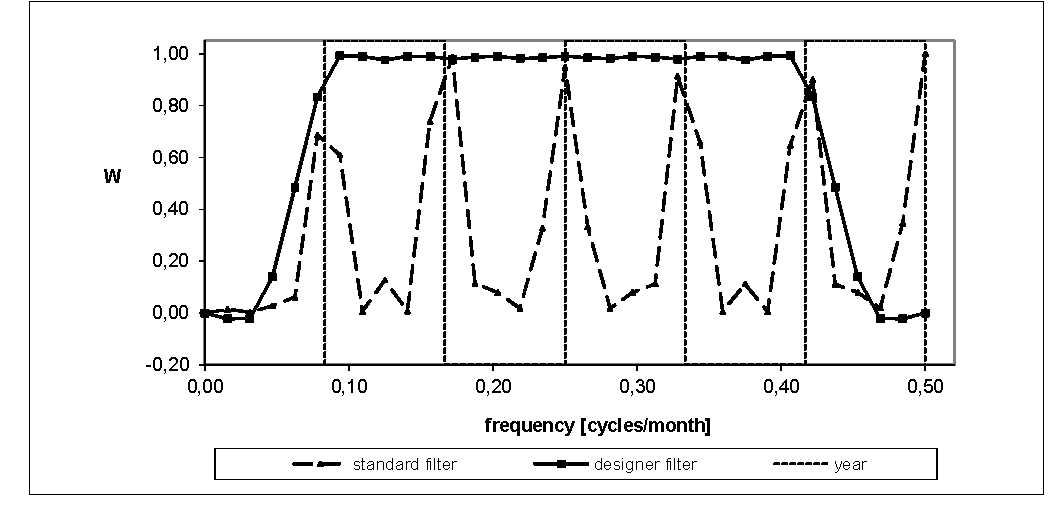
\includegraphics[width=\linewidth]{../images/capitolo2/filters.pdf}
 \caption{The band-pass filter designed for seasonal adjustment. Dashed line indicates the standard filtering. Vertical dashed line indicates integer multiples of 1 cycle/year.}
 \label{fig:filters}
\end{figure}
The weights $w_k$ that correspond to this filter of Figure \ref{fig:filters} are shown to 7 digits precision in Table \ref{tab:digits}. The weights \textit{w$_k$} for all the odd values of \textit{k} are identically equal to 0, as are the weights for $ k>18$. This set of weights satisfies the various constraints mentioned in this section. The additional property that the weights are zero for all odd values of\textit{ k} produces an additional advantage: the high frequency section of the spectrum can be determined in a very simple second step, which is evidently statistically independent. If \textit{y} is the time series from which the seasonal component has been removed with the above filter, then the high frequency component \textit{h} is obtained by taking:
\begin{equation}
h_i = (2 \tilde{y_i} - \tilde{y_i} - \tilde{y}_{i+1})/4
\end{equation}
Whereas the \textit{trend+cycle} time series \textit{c} (without high frequency contributions) is obtained from:
\begin{equation}
c_i = (2\tilde{y_i}+\tilde{y_i}+\tilde{y}_{i+1})/4
\end{equation}
With the weights of Table \ref{tab:digits} it is clear that after 18 months any seasonal adjusted time series \textit{y} will not change, when using this filter alone.\\
\bigskip
\begin{table}[h]
\captionof{table}{Filter weights for a band-pass filter designed to extract seasonal behaviour from a time series.}
\label{tab:digits}
\centering
\begin{tabular}{r r}
k & $w_k=w_{-k}$\\
\hline
0 & 0,7358026\\
2 & -0,2219532\\
4 & -0,1504270\\
6 & -0,0659661\\
8 & 0\\
10 & 0,0309203\\
12 & 0,0302373\\
14 & 0,0143577\\
16 & 0\\
18 & -0,0050703\\
\hline
\end{tabular}
\end{table}
Given that applying this filter to any given time series is as straightforward as the more standard filtering steps (such as applying Henderson filter for smoothing a time series) there is no fundamental difficulty in incorporating this weight system in the standard packages that are currently widely available. By doing this, for instance, with the X-13-ARIMA package, all the other tools that this package offers are still available.
\begin{figure}[h]
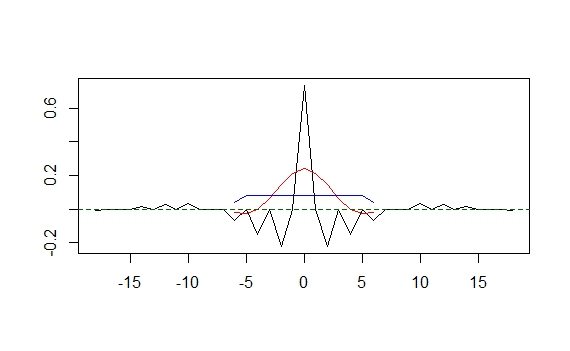
\includegraphics[width=\linewidth]{../images/capitolo2/henderson_designed_ma.jpeg}
\caption{Time-domain representation of different filters. Black line is the designed filter, ranging in a [-18:18] terms width; red line indicates the Henderson 13-terms filter and blue line indicates the 13-terms seasonal moving average filter.}
\label{fig:henderson_designed_ma}
\end{figure}
A possible alternative is to pre-process time series with this filter, and this is exactly the procedure proposed in this paper. There is no loss of information in this pre-processing step since the seasonal factor and the \textit{trend+cycle+noise} series are both available and their sum is identical to the original time series. The time series filtered with the proposed weight system can then be provided as input for the standard packages (in this case, those available in JDemetra+), in order to be able to use the extensive toolset of those packages for a more detailed analyses of the character and causality of the seasonal factor. Such more in-depth analyses could be ``off-line'' and would not interfere with the normal publishing schedules of the original and seasonal adjusted time series.\\
Figure \ref{fig:henderson_designed_ma} plots the two mentioned set of filters represented in the time domain, comparing them with the function of the designed one.
\subsection{Periodogram}
Time series are generally presented in the time domain. Another interesting representation of the same series is in the frequency domain, considering that any stationary time series can be expressed as a combination of sinusoidal functions, thanks to the Fourier transform. It represents the spectrum, and its representation is called the periodogram. It is possible to obtain it as follows:
\begin{equation}
y_t = \sum\limits_{i=1}^{\frac{n}{2}}[\beta_{1_{i}}\cos(2\pi\omega_{i}t) + \beta_{2_{i}}\sin(2\pi\omega_{i}t)]
\end{equation}
The $\beta$'s work as regression parameters, obtained from: $\beta_{1_{i}}=A_{i} \cos(\phi_{i})$ and $\beta_{2_{i}}=-A \sin(\phi_{i})$, where $\phi$ is called the phase. It determines the starting point (in degrees) for the cosine wave. A is the amplitude.\\Fourier analysis inspects historical data in the frequency domain, in order to evaluate how cycles of different frequencies influence the behaviour of \textit{y$_t$}. Indeed, dominant cycles of a time series are clearly highlighted by the periodogram, i.e. a high peak at a certain frequency indicates a dominant cyclical behaviour with a certain periodicity in a time series . The periodicity \textit{P} of a phenomenon is related to its frequency $\omega$: $P=2 \pi / \omega$. It means that for a monthly series, seasonal frequencies are $\pi/6$, $\pi/3$, $\pi/2$, $2\pi/3$, $5\pi/6$ and $\pi$, and they correspond to 1, 2, 3, 4, 5 and 6 cycles per year (for quarterly sampled series, the two seasonal frequencies are $\pi/2$; one cycle per year, and $\pi$; two cycles per year).\\Also the trading day effect could have an influence in a periodogram. As a daily component, it repeats every seven days, so it goes through 4.348 cycles in a average month, which has 30.4375 days. Actually, this frequency (4.348) is higher than the Nyquist frequency. If any signal has a frequency higher than $\omega_{N_{yq}}$, it is an aliasing signal, i.e. it is indistinguishable from a lower-frequency signal. When this happens, the signal “appears” with much lower $\omega$. Consequently, the $\omega=4.348$ appears, for monthly data, as 0.348, which is the trading day frequency. A more detailed discussion of the trading days effect identification and its spectral diagnostic is offered by \citep{fineal1999}.\\When a time series is dominated by a strong seasonal factor, it has peaks at the seasonal frequencies, whereas a seasonally adjusted time series should have no peaks at those frequencies. Moreover, the presence of the trend component is always evidenced by a peak at frequency zero and so, when a periodogram has high values at low frequencies, i.e. at $(0 \leq \omega \leq 0.06)$, the long-term component influences significantly the series. On the contrary, if high values of the periodogram concentrate more at high frequencies, the time series is rather trendless and its irregular component is relevant.\\JDemetra+ contains different spectral diagnostics. First, it is possibile to obtain a spectral plot of the raw time series, obtained (by default) after the performance of a first difference operation on the time series, to get the data stationary. Indeed, non-stationarity of a series could lead to a misinterpretation of the periodogram.  One other issue is related to the presence of outliers, since they can influence the outcome of the periodogram as well. This is why a pre-transformation of data is advisable, as done by both TRAMO/SEATS and X-13-ARIMA.  As is visible from Figure \ref{fig:raw}, in JDemetra+ the seasonal frequencies are marked as grey vertical lines, while the bordeaux line represents the trading day frequency.
\begin{figure}[h]
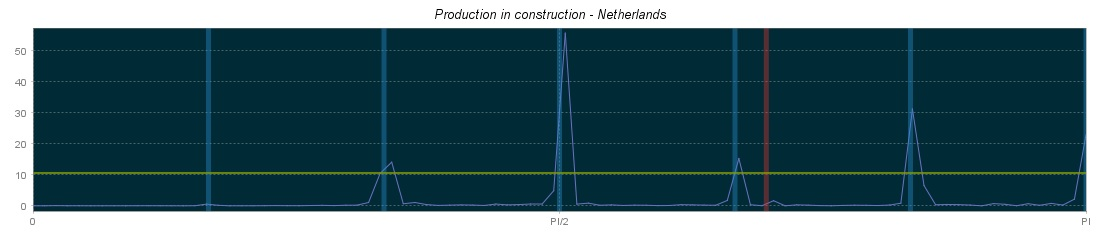
\includegraphics[width=\linewidth]{../images/capitolo2/raw.jpg}
\caption{JDemetra+ representation of a periodogram.}
\label{fig:raw}
\end{figure}
In addition to the ‘raw’ periodogram, once the seasonal adjustment procedure has been carried out, JDemetra+ offers some spectral diagnostics. Especially, it is possible to obtain periodograms of the seasonally adjusted series, residuals and irregular component. Further details will be given in the next section.
\section{Seasonal adjustment procedure}
The time series used in this study represents the air passenger movements registered at the Schipol airport in Amsterdam, the Netherlands. The series covers a length of 196 monthly registrations, spanning the period from January 1999 to April 2015. As illustrated in Figure \ref{fig:series}, the data present a strong seasonal pattern, which is slightly varying over the entire series.
\begin{figure}[h]
 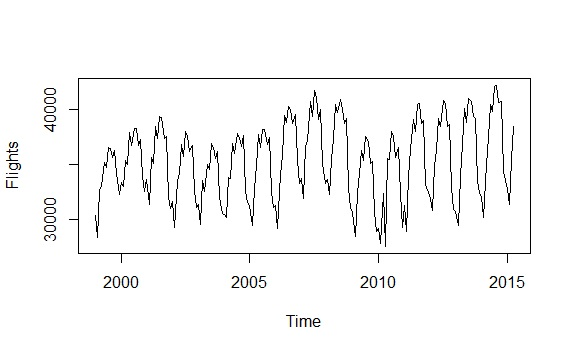
\includegraphics[width=\linewidth]{../images/capitolo3/series.jpg}
 \caption{Amsterdam Schipol airport flights from January 1999 to April 2015.}
 \label{fig:series}
\end{figure}
\subsection{JDemetra+}
The first step is to carry out a seasonal adjustment with JDemetra+, i.e. with TRAMO/SEATS and X-13-ARIMA procedures, without any pre-filtering treatment of the series. The software offers the possibility, through its \textit{workspace} window, to choose between different pre-defined \textit{specifications} implemented in the two methods. Those \textit{specifications} are sets of parameters and values assigned to them that contain all the necessary information for seasonal adjustment and for modelling the time series during the pre-decomposition step. Table 3.1 reports all the possible specifications (the first seven are about TRAMO/SEATS, the last six about X-13-ARIMA), but it is important to highlight two main points. First, the user has the option to set manually those parameters, depending on the nature of the analysis. Second, this paper will focus on the default specifications settled by JDemetra+ (\textit{RSAful}l for TRAMO/SEATS and \textit{RSA4c} for X-13-ARIMA), but with a fixed model parameters choice, the so called ARIMA ``Airline Model'' (0,1,1)(0,1,1) (Box and Jenkins, 1976), one of the most commonly used seasonal ARIMA model, in order to meet the parsimony principle. The \textit{Transformation} column indicates the performance of a test to choose between an additive decomposition (no transformation) and multiplicative decomposition (logarithmic transformation) of the time series. Concerning the ARIMA model selection, the acronym AMI stands for Automatic Model Identification. A detailed discussion of different parameters and specifications can be found in \citep{gru2015}.
\begin{figure}[h]
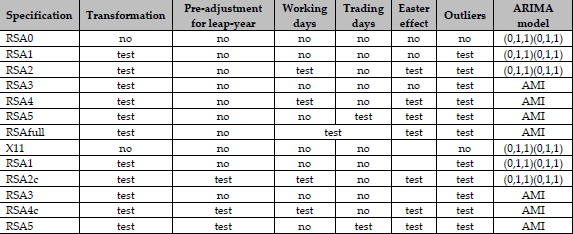
\includegraphics[width=\linewidth]{../images/capitolo3/specification.jpg}
\caption*{Table 3.1 \quad TRAMO/SEATS and X-13-ARIMA pre-defined specifications.}
\label{fig:specification}
\end{figure}
The software performs an automatic identification of the calendar effects of a time series, and includes them as regressors in the RegARIMA model fitted in the \textit{modelling} part. This paper will not offer a thorough discussion about these regression parameters, i.e. outliers, Easter effect, trading/working days effect, leap-year effect; for it will mainly focus about the Fourier-domain representation of the historical data. In this case study, this determinist effects identification will not be modified from the automatic one performed by the software.
\subsection{JDemetra+ spectral analysis}
A helpful tool implemented in JDemetra+ refers to the spectral analysis of time series. The possibilities for a spectral analysis offered by the software are Periodogram, Auto-regressive Spectrum and Tukey Spectrum. This paper will focus only on the periodogram. Figure \ref{fig:amsper} presents the periodogram of the analysed historical data. As mentioned in Section 2, the JDemetra+ periodogram applies a first difference operation on data. As in most of the JDemetra+ tools, users are free to change this setting, by increasing the differencing order or deleting it. JDemetra+ points out the significance of a peak by a green horizontal line, which denotes the 0.05 significance level.
\begin{figure}[h]
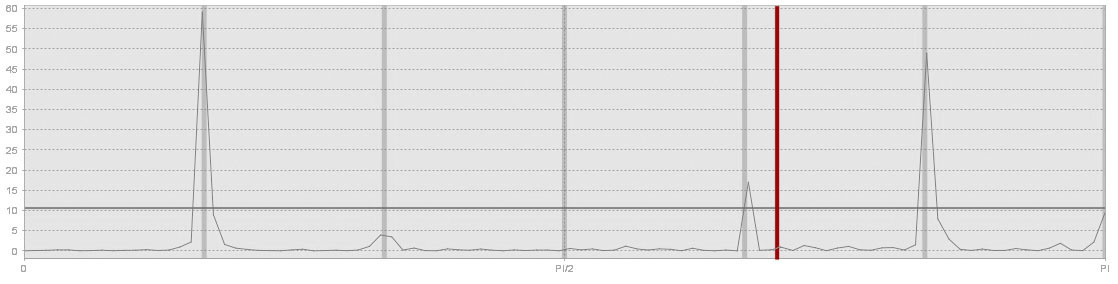
\includegraphics[width=\linewidth]{../images/capitolo3/amsper.jpg}
\caption{Periodogram of unadjusted time series.}
\label{fig:amsper}
\end{figure}
The unadjusted series shows a peak at the first seasonal frequency, which means the presence of a strong seasonal movement of one cycle per year. Another significant peak coincides with the fifth seasonal frequency, related to a movement of five cycles per year. This periodogram gives results which could be visible also from the simple plot of the series (the presence of seasonality), but from this frequency-domain representation it is more straightforward to check the cycles of the dominant seasonal movements.\\When starting a seasonal adjustment with JDemetra+, both the methods imply two steps; a \textit{modelling} part and a \textit{decomposition} part. As briefly discussed in the introduction, the \textit{modelling} part consists of identifying the regression parameters that have a deterministic effect on the data, and then of fitting an ARIMA model to the data, to give a suitable model for an acceptable decomposition. Since this paper focuses on the designed filter to decompose a time series in its components, it does not offer detailed discussion of the \textit{modelling} results, but rather on the spectral diagnostics of the decomposition output and the filtering procedures. For an exhaustive discussion about the \textit{modelling} part see \citep{tramo2008}. Indeed, JDemetra+ offers several diagnostics, using a user-friendly graphic for the results of the various tests. Together with every \textit{p.value} associated to each test, an evaluation of the result is given in words (good, uncertain, severe) coloured, respectively, in green, yellow and red. This helps for interpretation of the results.\\
\subsection{TRAMO/SEATS and X-13-ARIMA spectral diagnostics}
Once the seasonal adjustment has been performed, JDemetra+ evaluates the quality of the decomposition through a wide range of diagnostics. Within these, a \textit{spectral diagnostic} consists in three frequency-domain charts, one for the model residuals, one for the irregular component, and one for the seasonally adjusted series. Actually, the software offers these diagnostics both as periodogram and as auto-regressive spectrum, but only the periodograms are considered here. Figure \ref{fig:perRES} plots the periodogram of the residuals. In this latter, when a peak occurs at a seasonal or at the trading day frequency, it means that the choosed model does not fit well the data. Respectively, peaks at seasonal frequencies highlight an inappropriate filter choice for the decomposition of the series, while a peak at the trading day frequency suggests a wrong identification of the deterministic effects used as regression variables in the RegARIMA model.
\begin{figure}[h]
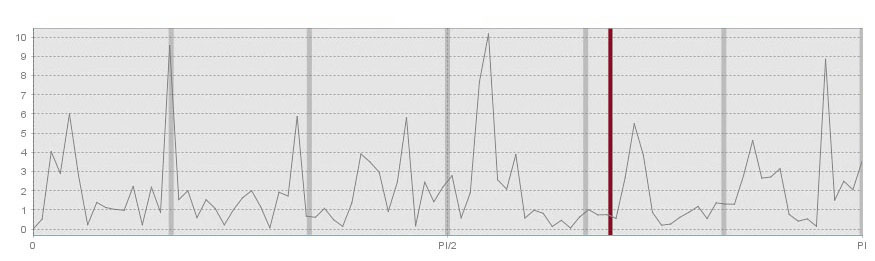
\includegraphics[width=\linewidth]{../images/capitolo3/perRES.jpg}
\caption{TRAMO/SEATS residuals periodogram.}
\label{fig:perRES}
\end{figure}
In the periodogram of residuals obtained from TRAMO/SEATS,  no peak exceeds the significance level, even if some movement is present through different frequencies; particularly, a peak is visible at the first seasonal frequency.\\In a periodogram of seasonally adjusted series or of the irregular component, a peak at any seasonal frequency denotes the possible inadequacy of the filters for the time interval considered for the spectrum estimation.\\For computational reasons, for the seasonally adjusted series and irregular component periodograms, JDemetra+  does not provide the green horizontal line that highlights peaks above the significance level. In the adjusted series (figure \ref{fig:perIRRSA}, lower chart), the periodogram does not show any peak at seasonal frequencies, reflecting a good decomposition of the original series performed by SEATS and a satisfactory removal of the seasonal effect. As desirable, low frequencies have low amplitudes, while higher values are registered at higher frequencies, in between the seasonal harmonics. Indeed, the noise component is not totally removed, as can be seen in the upper chart of Figure \ref{fig:perIRRSA}, related to the irregular periodogram, which shows relevant power between seasonal frequencies.
\begin{figure}[h]
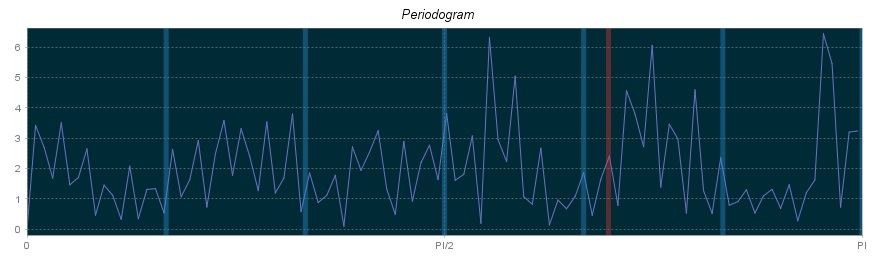
\includegraphics[width=\linewidth]{../images/capitolo3/perIRR.jpg}
\end{figure}
\begin{figure}[h]
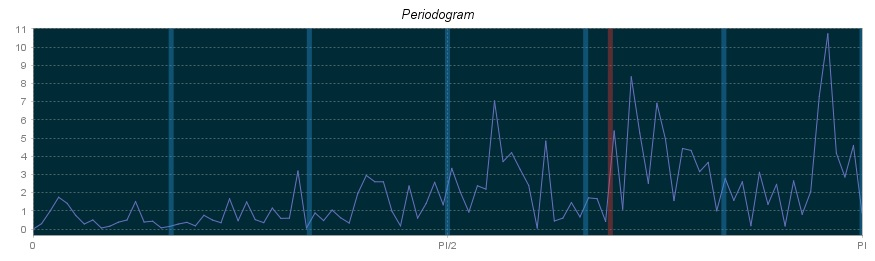
\includegraphics[width=\linewidth]{../images/capitolo3/perSA.jpg}
\caption{TRAMO/SEATS irregular (top) and seasonally adjusted series (bottom) periodograms.}
\label{fig:perIRRSA}
\end{figure}
In the next section, about the seasonal adjustment of the filtered series, these same plots will show a much smoother behaviour. In the following charts are reported the same three periodograms, but the ones obtained from the X-13-ARIMA procedure, which makes the use of 3x3 seasonal filter and a 13-terms Henderson moving average as trend filter. The length of these filters depends on the time series, and the selection is done automatically by the X-11 algorithm \citep{dageal1996}. For the comprehension of the length selection criterion, see also \citep{gru2015}, while a brief discussion about the role of these filters in standard filterng procedures is provided in the Appendix. Periodograms in Figure \ref{fig:X13per} show a similar behaviour to the ones obtained from TRAMO/SEATS, and their interpretation is the same. 
\begin{figure}[h]
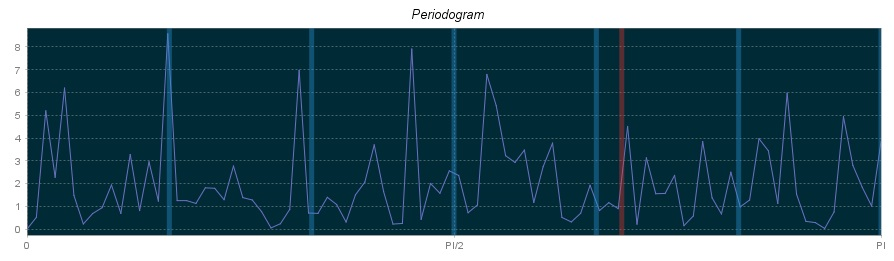
\includegraphics[width=\linewidth]{../images/capitolo3/XperRES.jpg} 
\end{figure}
\begin{figure}[h]
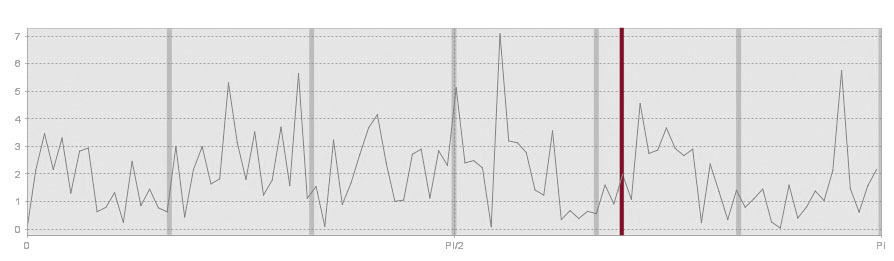
\includegraphics[width=\linewidth]{../images/capitolo3/XperIRR.jpg} 
\end{figure}
\begin{figure}[!h]
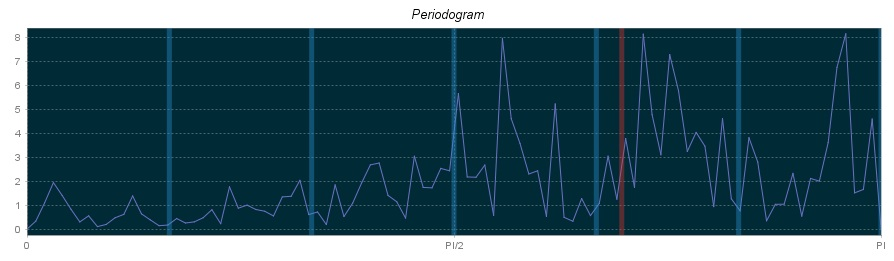
\includegraphics[width=\linewidth]{../images/capitolo3/XperSA.jpg} 
\caption{X-13-ARIMA residuals (top), irregular (middle) and seasonally adjusted (bottom) series periodograms.}
\label{fig:X13per}
\end{figure}
\subsection{Squared gain of components filter.}
TRAMO/SEATS estimates the various components using the so-called Wiener-Kolmogorov filters. These filters are symmetric. It means that observations from the past and from the future have to exist, so there is the need for forecasts and backcasts for the both ends of the series. This operation is performed through the ARIMA model estimated by TRAMO. Further discussion about these filters is provided in the Appendix.\\An interesting tool related to the quality of the decomposition is the square gain of the components filter. The latter indicates which frequency components are suppressed or amplified by the filtering operation. The derivation of the squared gain function is briefly discussed in the Appendix. If in a frequency band the squared gain of a filter has value zero, then that filter passes no movement from this range of frequencies to the output series. On the other hand, when its value is equal to one, all the movement from that range is delivered to the component estimator. It means that the squared gain of an optimal seasonal component estimator filter should have unitary values at seasonal frequencies, and zero in between the same frequencies. On the contrary, for the seasonally adjusted series filter, this function should have values equal to zero at those same frequencies. In general, the squared gain shape depends on the model for the time series. A thorough explanation of the derivation of the squared gain function and its interpretation, as the values of the parameters of the ARIMA model and the length T of the series change, is discussed in \citep{fineal2006}.
\begin{figure}[h]
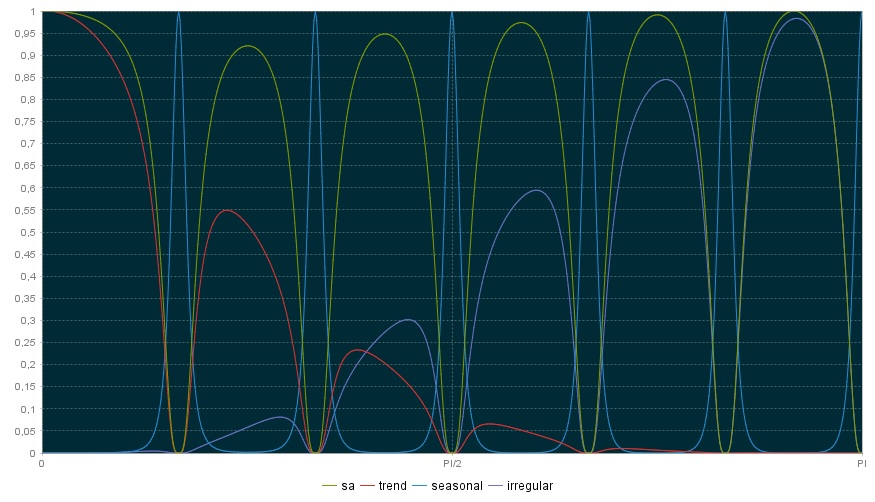
\includegraphics[width=\linewidth]{../images/capitolo3/squaredgain.jpg}
\caption{Squared gain of TRAMO/SEATS components filters}
\label{fig:squaredgain}
\end{figure}
Figure \ref{fig:squaredgain} represents the squared gain of the components filters obtained by TRAMO/SEATS from the dataset analysed in here. As the value for seasonal component estimator is equal to one at seasonal frequencies, the decomposition procedure seems to act quite well, with relatively narrow troughs. On the other hand, the shape of the squared gain of the seasonally adjusted component filter seems to miss some signal between seasonal frequencies, and it does not reach the exact value of one. It will be interesting, in the next section, to compare this squared gain chart to the one obtained from the same time series, but pre-filtered with the proposed filter.
As X-13-ARIMA makes use of the algorithm of X-11, which implies the use of standard filters (seasonal moving average and Henderson filters, where only the filter length may vary), JDemetra+ does not offer a squared gain representation of these filters, but only for the TRAMO/SEATS ones, since they are different for each analysed time series.
\section{Filtering a time series with the designed filter}
\subsection{First iteration of the designed filter on a time series}
The filtering of the time series using the filter proposed in Section 2 has been performed with the statistical software R. The decompostion of the time series through the filtering operation is represented in Figure \ref{fig:collage}.
\begin{figure}[h]
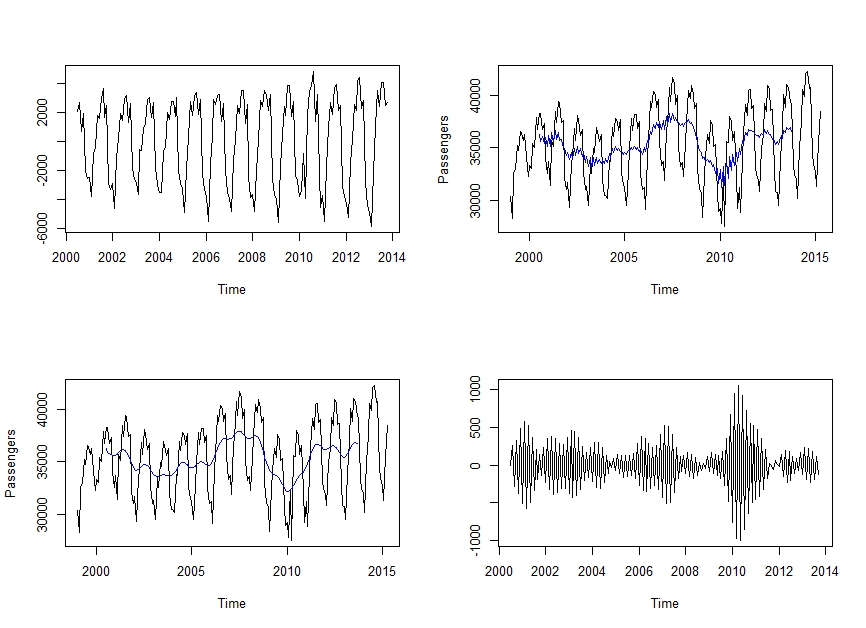
\includegraphics[width=\linewidth]{../images/capitolo4/collage.jpeg}
\caption{Decomposition of the time series with the proposed filter.}
\label{fig:collage}
\end{figure}
The upper-left panel of Figure \ref{fig:collage} represents the seasonal component, obtained with a single iteration of the designed filter through equation (7). Then, this component has been subtracted from the original series, in order to obtain the \textit{trend+cycle+noise} series, represented in the upper-right panel (blue line) in a comparison with the unadjusted data (black line). It is worth to highlight again that the sum of this \textit{trend+cycle+noise} and the seasonal factor is identical to the original time series. According to equation (13), it is then straightforward to identify the high-frequency (noise) component and then to subtract it from this \textit{trend+cycle+noise} series. The pure smooth \textit{trend+cycle} component (the one in blue as well) is compared again to the original data (black line) in the bottom-left panel. Finally, the bottom-right chart reveals the high frequencies component, i.e. the ``noise'' of the series, which shows a strong increase in amplitude in the year 2010. Actually, an explanation of this increase could be the two additive outliers detected by both TRAMO/SEATS and X-13-ARIMA in this year, in the months of April and of December.\\The outcome of the seasonally adjusted data is not totally satisfactory. While clearly a great amount of the seasonal pattern is removed, the visual impression is that the filtering has not been completely successful. One of the reasons for this is the strong amplitude of the seasonal component. One could deal with this in a number of different ways. One possibility is simply to repeat the filtering process, but since the aim of this study is the analysis of the output of the seasonal adjustment procedure with the filtered series as input, the second filtering operation will be not performed in here. Figure \ref{fig:tc_periodogram} plots the JDemetra+ periodogram of the time series filtered, through R, with the proposed filter, before the performance of the further seasonal adjustment. This time, as opposed to what was done in Section 3, there is no need for differencing the time series, since it is already stationary. Therefore, the first difference operation has been removed.
\begin{figure}[h]
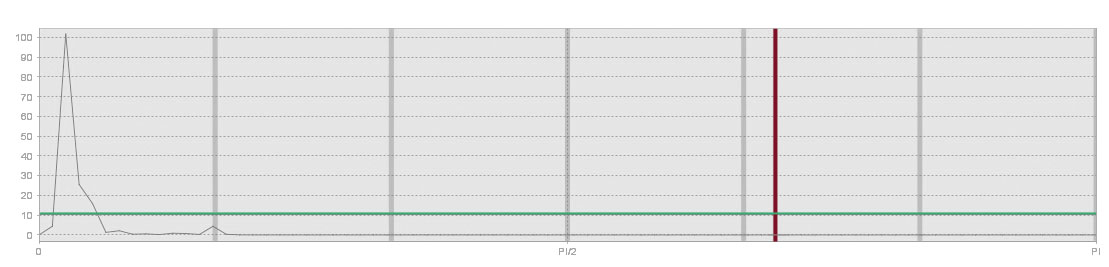
\includegraphics[width=\linewidth]{../images/capitolo4/tc_periodogram.jpg}
\caption{Filtered time series periodogram.}
\label{fig:tc_periodogram}
\end{figure}
As a proof of the imperfect seasonality removal, a peak is visible at the first seasonal frequency of $\sim$ 1/12 cycle/month. This imperfect removal after one pass of the filter is due to the fact that the frequency of $\sim$ 1/12 cycle/month is near the edge of the band which the seasonal filter removes. The removal is therefore slightly less than 100\%, which will leave a noticeable residual for a signal with a very strong annual variation. One could try to deal with this by making the band to be removed slightly broader, but this would imply that there would also be some undesirable suppression of genuine longer term cycle behavior. Another option might be to try to produce a sharper transition in the band-pass filter from the region in the spectrum where it passes all signal to the region in the spectrum where all signal is blocked. While this is possible, the effect it has is that in the time domain the linear coefficients of the filter function are non-zero over a larger range. In practice there is always a trade-off between the level to which seasonal behaviour can be suppressed in the time series for \textit{trend+cycle+noise}, and the range over which the filter function has non-zero values. Apart from this limitation, the periodogram has values equal to zero for all the frequencies after the first seasonal one. It means that the removal of the seasonal component through the designed filter works properly for all the other harmonics. To confirm the efficacy of the seasonal removal, it is possible to compare this periodogram to the one in Figure \ref{fig:perIRRSA} and \ref{fig:X13per}, of the seasonally adjusted series obtained through TRAMO/SEATS and X-13-ARIMA.\\
\subsection{Filtered series as input for JDemetra+ analysis}
The filtered time series (the \textit{trend+cycle} series represented in bottom-left chart of Figure \ref{fig:collage}) has been used as input for a JDemetra+ analysis. On some occasions, TRAMO provides a not decomposable model. It happens when components have a negative spectrum for some frequencies. It is then said that the model presents a “non-admissible” decomposition. When this happens, SEATS automatically modifies the model parameters, searching for a decomposable model that is not far from the one identified by TRAMO. The search always converges. For a more extensive discussion, see \citep{mar2008}. This is the case of the TRAMO/SEATS analysis performed on the filtered series, which finds the TRAMO model not decomposable. As mentioned in Section 3, the considered models is the (0,1,1)(0,1,1) ARIMA model.\\ Before comparing the spectral analysis of the outputs, it is worth to compare the seasonal factors obtained from the JDemetra+ decomposition performed on the filtered data and on the non-filtered data. Relevant is the difference in the amplitude of the seasonal factor. The lower chart of Figure \ref{fig:X13_seas}, of the not filtered data, shows an amplitude ranging between -6000 and 4000. The seasonal factor component of the filtered data (upper chart) shows a trend either smoother (at the peaks) and lower, ranging between -400 and 400.\\In the following charts are represented the spectral diagnostics of the output of the TRAMO/SEATS method, obtained when using the filtered series as input for the seasonal adjustment.
\begin{figure}[H]
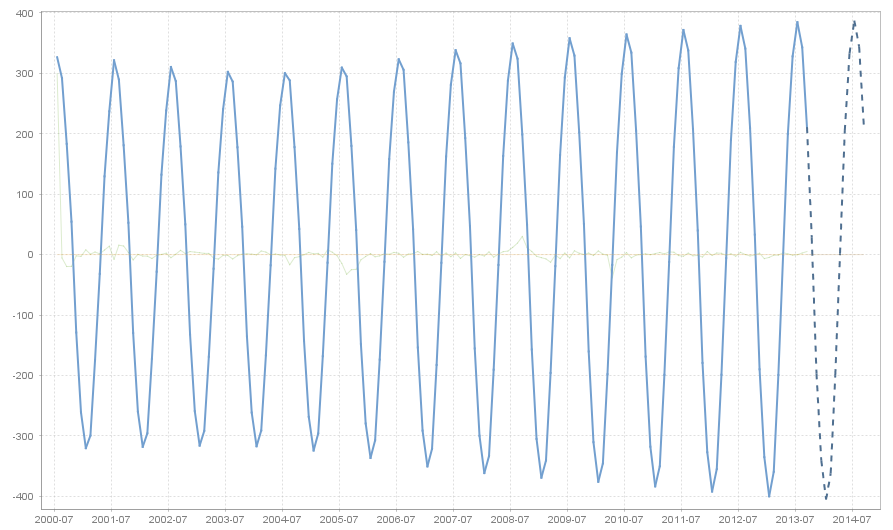
\includegraphics[width=\linewidth]{../images/capitolo4/X13_seas_cmp_filtered.jpg}
\end{figure}
\begin{figure}[H]
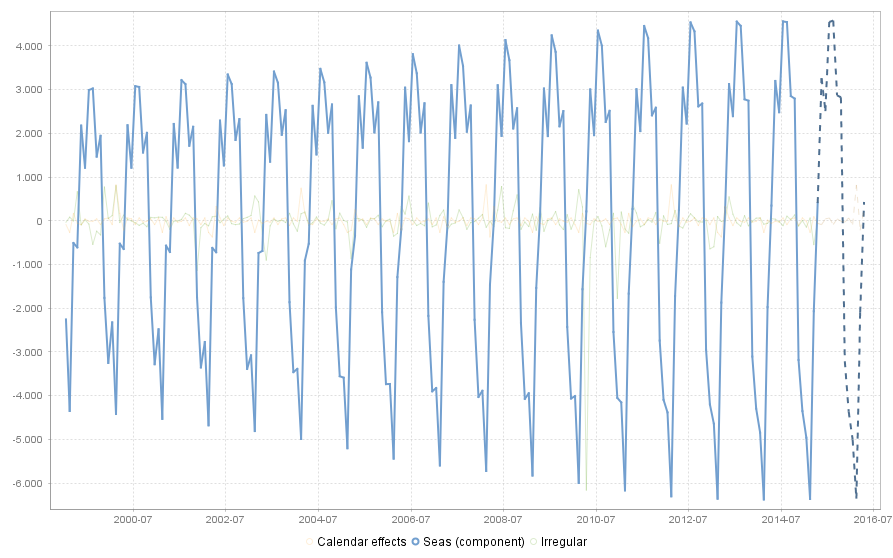
\includegraphics[width=\linewidth]{../images/capitolo4/X13_seas_cmp_plan.jpg}
\caption{Comparison of seasonal factors obtained through X-13-ARIMA decomposition (TRAMO/SEATS acts similar).}
\label{fig:X13_seas}
\end{figure}
\begin{figure}[H]
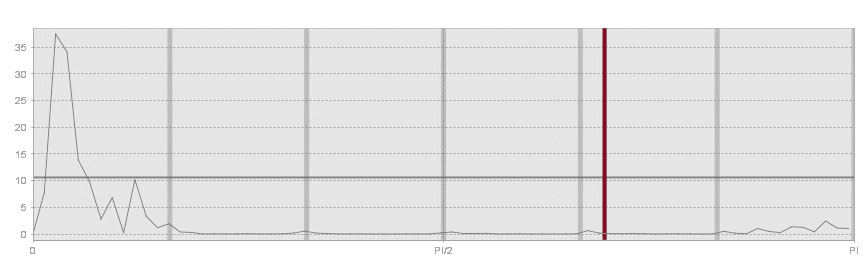
\includegraphics[width=\linewidth]{../images/capitolo4/TSresper.jpg}
\end{figure}
\begin{figure}[H]
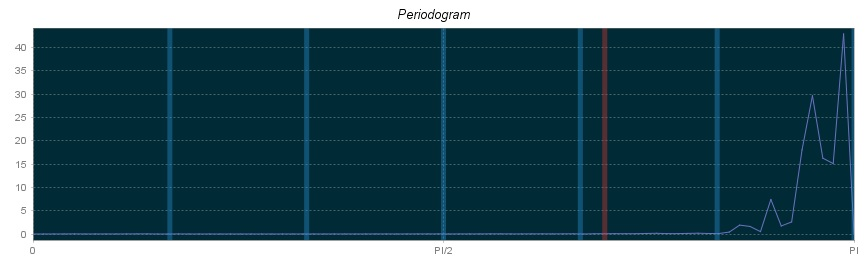
\includegraphics[width=\linewidth]{../images/capitolo4/TSirrper.jpg}
\end{figure}
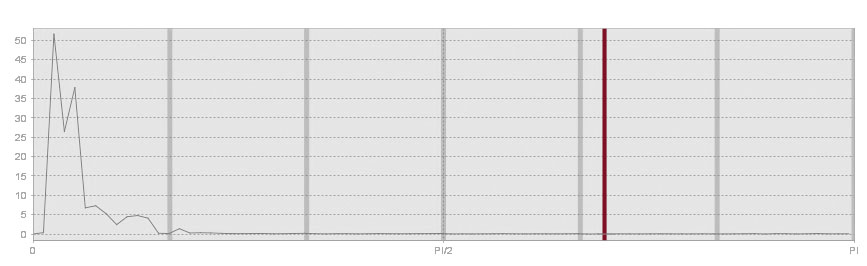
\includegraphics[width=\linewidth]{../images/capitolo4/TSsaper.jpg}
\begin{figure}[H]
\caption{Residuals (top), irregular (middle) and seasonal adjusted (bottom) periodograms obtained by TRAMO/SEATS.}
\label{fig:TSperr}
\end{figure}
The most relevant result about these periodograms is the total absence of power at any seasonal frequency. This is a proof of the efficacy of the designed filter, particularly when the filtered series is used as input for further analysis. The comparison between Figure \ref{fig:TSperr} and the periodograms analyzed in Section 3 confirms this. Periodograms obtained from X-13-ARIMA show a similar behaviour to the TRAMO/SEATS ones, and therefore they will not be reported in here.\\JDemetra+ offers many other diagnostics. Some of them are related to the presence of seasonality. As a proof of the removal of the seasonal component, Table 4.1 represents the results of these tests (for both the procedures), whose check for the presence of seasonality in the seasonally adjusted series. An explanation of these tests is offered by \citep{gru2015}. As desirable, they testify the efficient removal of the seasonal factor from the time series.
\begin{figure}[h]
\label{fig:test}
  \begin{minipage}[b]{0.5\textwidth}
    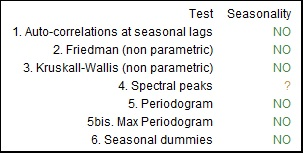
\includegraphics[width=\linewidth]{../images/capitolo4/testTS.jpg}
  \end{minipage}
  \hfill
  \begin{minipage}[b]{0.5\textwidth}
    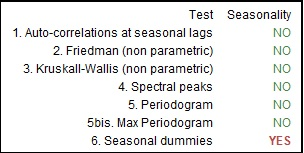
\includegraphics[width=\linewidth]{../images/capitolo4/testX13.jpg}
  \end{minipage} 
  \caption*{Table 4.1 \quad JDemetra+ output for tests about the presence of seasonality on seasonally adjusted series; TRAMO/SEATS on the left and X-13-ARIMA on the right.}
\end{figure}
When fitting a model to a time series, one of the most reliable indicators of the goodness of the fit is the Akaike Information Criterion (Akaike, 1974). When choosing between two different models, it is preferable to use the one with the lowest AIC value. This value in the two X-13-ARIMA procedures (the first one for the unadjusted data, the second one for the filtered data) is significantly different: it is respectively 2842.46 for the unadjusted time series and 1761.82 for the filtered time series.\\Figure \ref{fig:gainfilters} shows the squared gain of the components filters used by TRAMO/SEATS for the filtered time series decomposition. It is perfectly visible that the square gain of the seasonally adjusted filter (green line) catches much more signal if compared to the one of the unfiltered data, visible in Figure \ref{fig:squaredgain}, for it has value equal to one between the seasonal frequencies. It means that the seasonal component of the filtered data is much more deterministic than the one of the original data. To confirm this, the bright blue line, related to the seasonal factor filter, has value equal to zero for all the frequencies out of the seasonal ones. Furthermore, the squared gain of the trend filter (red line) has higher values for all the frequencies compared to the squared gain of the trend filter of Figure \ref{fig:squaredgain}. It means that all information about long term behavior is delivered to the output series.
\begin{figure}[h]
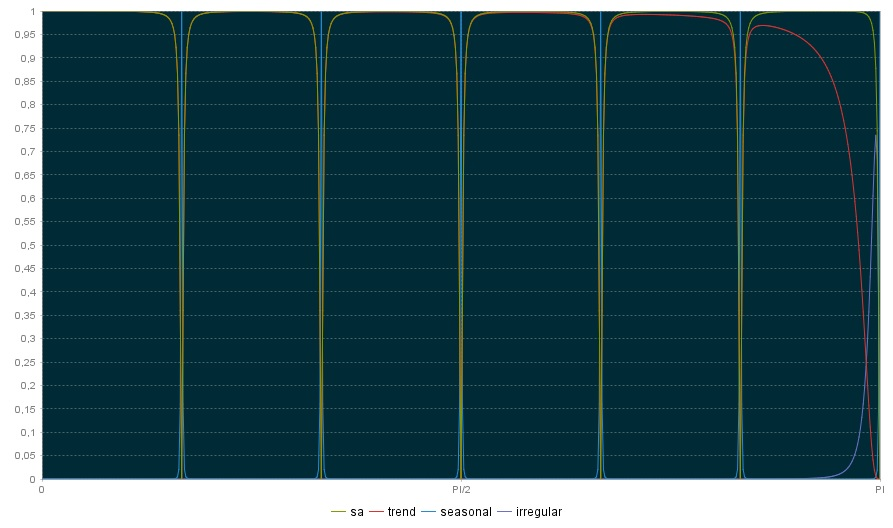
\includegraphics[width=\textwidth]{../images/capitolo4/gainfilters.jpg}
\caption{Squared gain of the components filters of TRAMO/SEATS procedure applied to filtered time series.}
\label{fig:gainfilters}
\end{figure}
\section{Conclusions}
It is possible to design linear filters for seasonal adjustment of time series that are more effective for real-time applications in official statistics than the filters currently in widespread use. Most packages already provide several options for filter coefficients, which means that it is straightforward to add the filter presented in this paper as another alternative.\\The advantage of the filter presented here is that the coefficients are non-zero over a range that is rather more restricted than the one obtained when recursively appying the existing naive options. This means that the resulting time series with seasonal adjustments can be finalised faster, and extrapolation towards the end points of time series is better constrained since it needs to take place over a much more limited range.\\An additional benefit of filtering all signals in a frequency band, is that this adjusts to a large degree for slow modulation of the amplitude of seasonal effects.\\The linearity of the filter together with the non-recursive formulation of it implies that partial time series can be adjusted for seasonal influences separately and then totalised which will by construction yield identical results to the seasonal adjustment of the summation of the partial time series.\\A JDemetra+ analysis of the output of this filtering operation confirms the aimed achievements. Particularly, the comparison between the seasonally adjusted data obtained through TRAMO/SEATS and X-13-ARIMA adjustments (see Figure \ref{fig:perIRRSA} and \ref{fig:X13per}) and the periodogram of the filtered series (Figure \ref{fig:tc_periodogram}) points out a more accurate removal of the seasonal factor and the irregular component for the time series filtered with the proposed filter. Even if the removal of the seasonal influences is not 100\% satisfactory, it is better than the adjustment obtained from the standard packages, and a second filtering operation with the same filter will give an output free of any seasonal movement. On the other hand, the identification and removal of the noise component is perfectly performed through equation (13), and the periodogram of filtered data shows no power at all at any high frequencies. Concerning the seasonal component, when using the filtered series as input for a seasonal adjustment procedure, the decomposition of the series leads to the identification of a seasonal factor for which the amplitude is largely reduced, if compared to the one obtained from a seasonal adjustment of the unfiltered data (see Figure \ref{fig:X13_seas}). \\The plots of the squared gain function of the filters components confirm a satisfactory performance of the proposed filter.
 \section*{Appendix}
 \subsection*{Standard filtering}
The standard initial filtering steps normally taken within the X-12-ARIMA package are threefold. In the first stepa provisional trend is identified by taking a moving average with the uniform weights and end-point correction, i.e. if the trend and cycle are indicated by \textit{c$_i$} then:
\begin{equation*}
c_i=\frac{1}{24}y_{i-6}+\frac{1}{12}y_{i-5}+...+\frac{1}{12}y_{i+5}+\frac{1}{24}y_{i+6}
\end{equation*}
In some literature this is referred to as $M_{2\times12}$ filter. This provisional trend is then subtracted from the time series to produce a provisional \textit{seasonal+irregular} component. At this stage the time series can be investigated for outliers which can be downweighted in a variety of ways. The next step is for each calendar month to calculate a moving average using the same month in several successive years. Often most weight is given to that month in the ``central'' year and symmetrically decreasing the weights for earlier or later years. Other options are available however.\\An updated \textit{trend+cycle+noise} series \textit{c} can now be computed, by subtracting the seasonal component that has just been determined from the original time series. This can be improved upon by once again applying a moving average filter, but rather than a uniform moving average, a Henderson filter is applied, which tapers more smoothly over the time series. In this way an updated \textit{trend+cycle+noise} is obtained which is the starting point also for obtaining an updated seasonal component. In principle one can iterate this process further.\\The combination of these individual filtering steps can also be expressed in terms of a single set of filtering weights since each individual step is simply a linear combination of the data with known weights. The combined steps described above tend to lead to a set of weights which is non-zero over a considerable range of months: [-84, 84] although the magnitude of these weights is generally only appreciable for the range [-40, 40].\\The implication of this is that for at least 40 months after any given reporting month the seasonal adjusted time series cannot be considered final, or even for 84 months if the full formal range of non-zero weights is taken into consideration. Further autoregressive modelling, if applied, will exacerbate this problem.
 \subsection*{Wiener-Kolmogorov filter}
The aim is to extract an estimate of a signal sequence $s(t)$ from an observable time series $y(t)$:
 \begin{equation*}
 y(t)=s(t)+\eta(t)
 \end{equation*}
where $\eta(t)$ is called noise. TRAMO/SEATS decomposition procedure works by means of the following algorithm.\\
An ARIMA model is fitted for the signal:
\begin{equation*}
\phi_{s}(B)s_{t}=\theta_{s}(B)a_{st} \quad \mbox{~where~} \quad a_{st} \sim w.n.(0,V_{s})
\end{equation*}
where the model for the time series is:
\begin{equation*}
\phi(B)y_{t}=\theta(B)a_{t} \quad \mbox{~where~} \quad a_{st}\sim w.n.(0,V_{a})
\end{equation*}
Notice: $\phi(B)=\phi_{s}(B)\phi_{\eta}(B)$, where B is the backshift operator ($B^j y_t=y_{t+j}$), and the $a_t$ are the white-noise innovations.\\The two polynomials $\phi(B)$ and $\theta(B)$ are, respectively, the stationary autoregressive polynomials in B and the invertible moving average polynomials in B, such that: 
\begin{equation*}
\phi(B)=(1-\phi_1 B-\phi_2 B^2-...-\phi_p B^p) \quad and \quad \theta(B)=(1-\theta_1 B-\theta_2 B^2-...-\theta_q B^q)
\end{equation*}
where $p$ and $q$ are the orders of the autoregressive and moving average polynomials.\\
Write:
\begin{equation*}
s_{t}=\Psi_{s}(B)a_{st}; \quad \Psi_{s}(B)=\frac{\theta_{s}(B)}{\phi_{s}(B)} ;
\end{equation*}
\begin{equation*}
y_{t}=\Psi(B)a_{t}; \quad \Psi(B)=\frac{\theta(B)}{\phi(B)} ;
\end{equation*}
The SEATS estimation of the signal $s$ at time $t$ then is:
\begin{equation*}
\hat{s_{t}}=\left ( \frac {V_{s}\Psi_{s}(B)\Psi_{s}(F)}{V_{a}\Psi(B)\Psi(F)} y_{t}\right )=v(B,F)y_{t}=\left ( v_{0}+\sum\limits_{j=0}^\infty  v_{j} (B^{j}+F^{j}) \right) y_{t}
\end{equation*}
Where F is the forward operator; $F=B^{-1}$; $F^{j}y_{t}=y_{t+j}$, and $v(B,F)$ is the so-called Wiener-Kolmogorov filter (WK).\\\textbf{Note}: if time series is stationaty, WK filter is equal to:
\begin{equation*}
v(B,F)=\frac{ACGF(s_{t})}{ACGF(y_{t})}
\end{equation*}
Wiener-Kolmogorov filters theory is based on the MMSE (Minimun Mean Square Error) idea. The filters derive from the observed model, which in turn depends on the time series. So, those filters differ depending on the observed series. WK filters are symmetric and bi-infinite; it means that for the ends of the series there is the need of forecasts and backcasts in order to get the estimations of those time points as well. This is performed by the TRAMO phase of seasonal adjustment, which provides an extended ARIMA model fitted to the data. Then, SEATS applies the WK filters.\\ With this procedure, highest weights are applied for central observations, even if the weighting pattern depends on the component to estimate. For example, for the seasonal component, highest weights are applied to the current value and the past and future values from the same period.
\subsection*{Square Gain of a filter}
It the context of filtering a series, it is possible to relate the spectral densities of the input $h_{y}(\omega)$ and of the output $h_{g}(\omega)$ as follows:
\begin{equation*}
h_{g}(\omega)=Y(\omega) h_{y}(\omega)
\end{equation*}
where $Y(\omega)$ represents the transfer function, in this case the Fourier Transform described in Section 2. The absolute value of the transfer function is the gain of the filter:
\begin{equation*}
G(\omega)=|Y(\omega)|
\end{equation*} 
and its power is the squared gain of the filter, which determines how the variance of the input contributes to the variance of the output at different frequencies.
\newpage

\bibliography{filter}

\end{document}
